\section{Evaluation}
\label{sec:eval}

\subsection{X-Server numbers}
\label{sec:x_eval}

An important part of our system is the X server to visualize and interact with the applications.  While our current design is somewhat limited in that it has too many layers of abstractions (using SDL as the backend), we have taken efforts to make the server run faster, which resulted in a much better user experience.  The biggest  performance improvement was moving from basic SDL to SDL-GLESv2 which improved the ``feel'' of X and the applications inside of it noticeably.  To try to capture this speed improvement we ran x11perf, which helps quantify the performance improvements.  As shown in Table \ref{tab:x_results}, there was noticeable improvements in a number of tests.
These tests we run from a Debian chroot, using localhost communication (not domain sockets) with the server, on the Palm Pre.  The tests were arbitrarily selected, with an attempt at finding representative ones.  These numbers should only be taken as illustrating the general performance improvements, not as an accurate measure of what real applications will be like.

\begin{table}[ht]
{\small
\hfill{}
\begin{tabular}{|l|c|c|c|}
\hline Benchmark & Xsdl & Xsdl-gles & \%Speedup \\ [2pt] 
\hline oddtilerect$100$ & $9950$ & $11500$ & $15.57\%$ \\ [2pt]
scroll$100$ & $6680$ & $7700$ & $15.26\%$ \\ [2pt]
copy$100$ & $2940$ & $3440$ & $17.01\%$ \\ [2pt]
rect$100$ & $15700$ & $18900$ & $20.38\%$ \\ [2pt]
fcircle$100$ & $8130$ & $9940$ & $22.26\%$ \\ [2pt]
ftext & $481000$ & $556000$ & $11.43\%$ \\ [2pt]
\hline 
\end{tabular}}
\hfill{}
\caption{ X server rendering with x11perf }
\label{tab:x_results}
\end{table}

\begin{figure}[tbh]
\centering
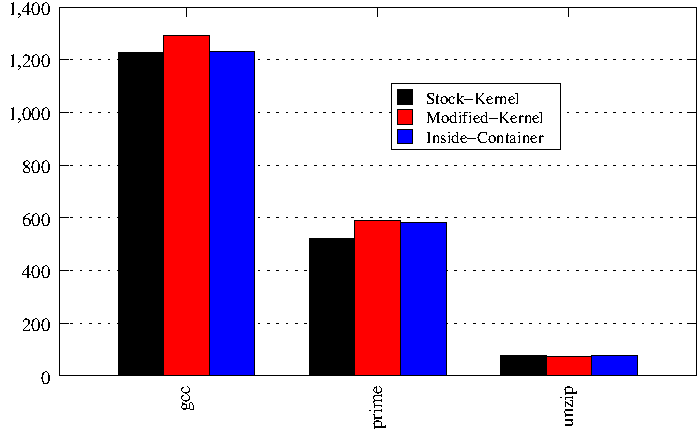
\includegraphics[width=1.0\columnwidth]{perf}
\caption{Running time comparison}
\label{fig:perf}
\end{figure}

\subsection{LXC Performance numbers}

Our addition of the linux container functionality to the kernel imposed no noticeable overhead to the phone.  Our testing (\ref{sec:lxc_perf}) and (\ref{sec:Quake}) proved that both the container kernel as well as the containers themselves, added no overhead to execution times.  More detailed testing with LMbench3 (\ref{sec:Lmbench3})proved that i/o, cpu, and memory performance were unaffected by the addition of the container code.  There was no overhead to running inside a container as well.  

\begin{figure}[tbh]
\centering
\includegraphics[width=1.0\columnwidth]{quake}
\caption{Execution Time for the Quake time-demo}
\label{fig:Quake}
\end{figure}

\begin{figure*}[bth]
\centering
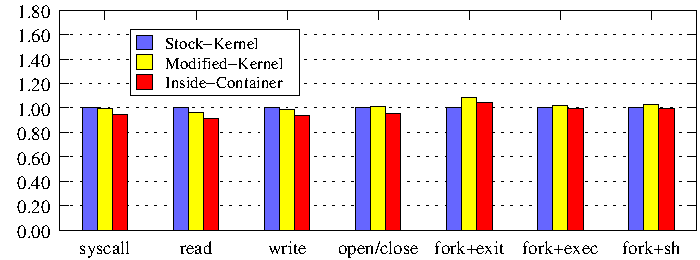
\includegraphics[width=1.0\columnwidth]{lmbench}
\caption{Normalized results from lmbench}
\label{fig:lmbench}
\end{figure*}

\subsection{LMbench3}
Our general benchmarks showed that there was no reduction in throughput with the addition of the containers.  We felt that more thorough testing was in order to determine if there was any overhead pertaining to latencies, context switching, and the file system.  LMbench3 is the most mature and commonly used among the LMbench family.  It runs a wide variety of tests, ranging from intensive latency testing of cache misses to extensive context switching testing.  LMbench has been heavily used in industry as well as acadamia \cite{lmbench}. \\

LMbench contains a suite of simple, portable benchmarks, comparing the performance of various UNIX systems.  It includes a variety of bandwidth benchmarks, of which the most popular are: cached file reads, memory operations (copy, read, and write), pipe, and TCP.  Additionally , it supports a wide variety of latency benchmarks, including: context switching, network connection establishment (pipe, TCP, UDP, RPC), file system operations (creates and deletes), process creation, handling of signals, system call overhead, and memory read latencies.  Lmbench also supports a variety of multiprocessor tests and includes large databases of results to compare one's results to. \cite{lmbench_paper}

\begin{figure*}[bth]
\centering
\includegraphics[width=1.0\columnwidth]{lmbench-files}
\caption{Normalized results from File System create/delete benchmarks in lmbench}
\label{fig:lmbench-files}
\end{figure*}
